\newpage

\section{Experiments with YOLO}
Looking at YOLO version 3, it has released two different convolutuional network arcitecture, one light and one normal. There is also a few models of the normal architecture, but they only differ in terms of resolutions inside the CNN. They are all trained on the same COCO dataset.

The different models of the YOLOv3, performance-wise differ in case of accuracy and time to compute.

In this example an image of my living room, who is a bit dark, got backlight is chosen as example since it should be a more difficult image to detect objects in.

The test were used on an older laptop CPU. Using the darknet test function as mentioned in chapter \ref{getYOLOgoing}.

\subsection*{YOLOv3-tiny}
The lightest version of YOLOv3.

Frame rate on fast GPU: 220 FPS \cite{yolo_res}.
\begin{lstlisting}[frame=single]
# Running YOLOv3 Tiny with threshold value of 10% 
# Input:
./darknet detect cfg/yolov3-tiny.cfg yolov3-tiny.weights data/stue.jpg -thresh 0.1

#Output
data/stue.jpg: Predicted in 3.294758 seconds.
laptop: 49%
tvmonitor: 73%
sofa: 16%
chair: 18%
\end{lstlisting}

\begin{figure}[h]
    \centering
        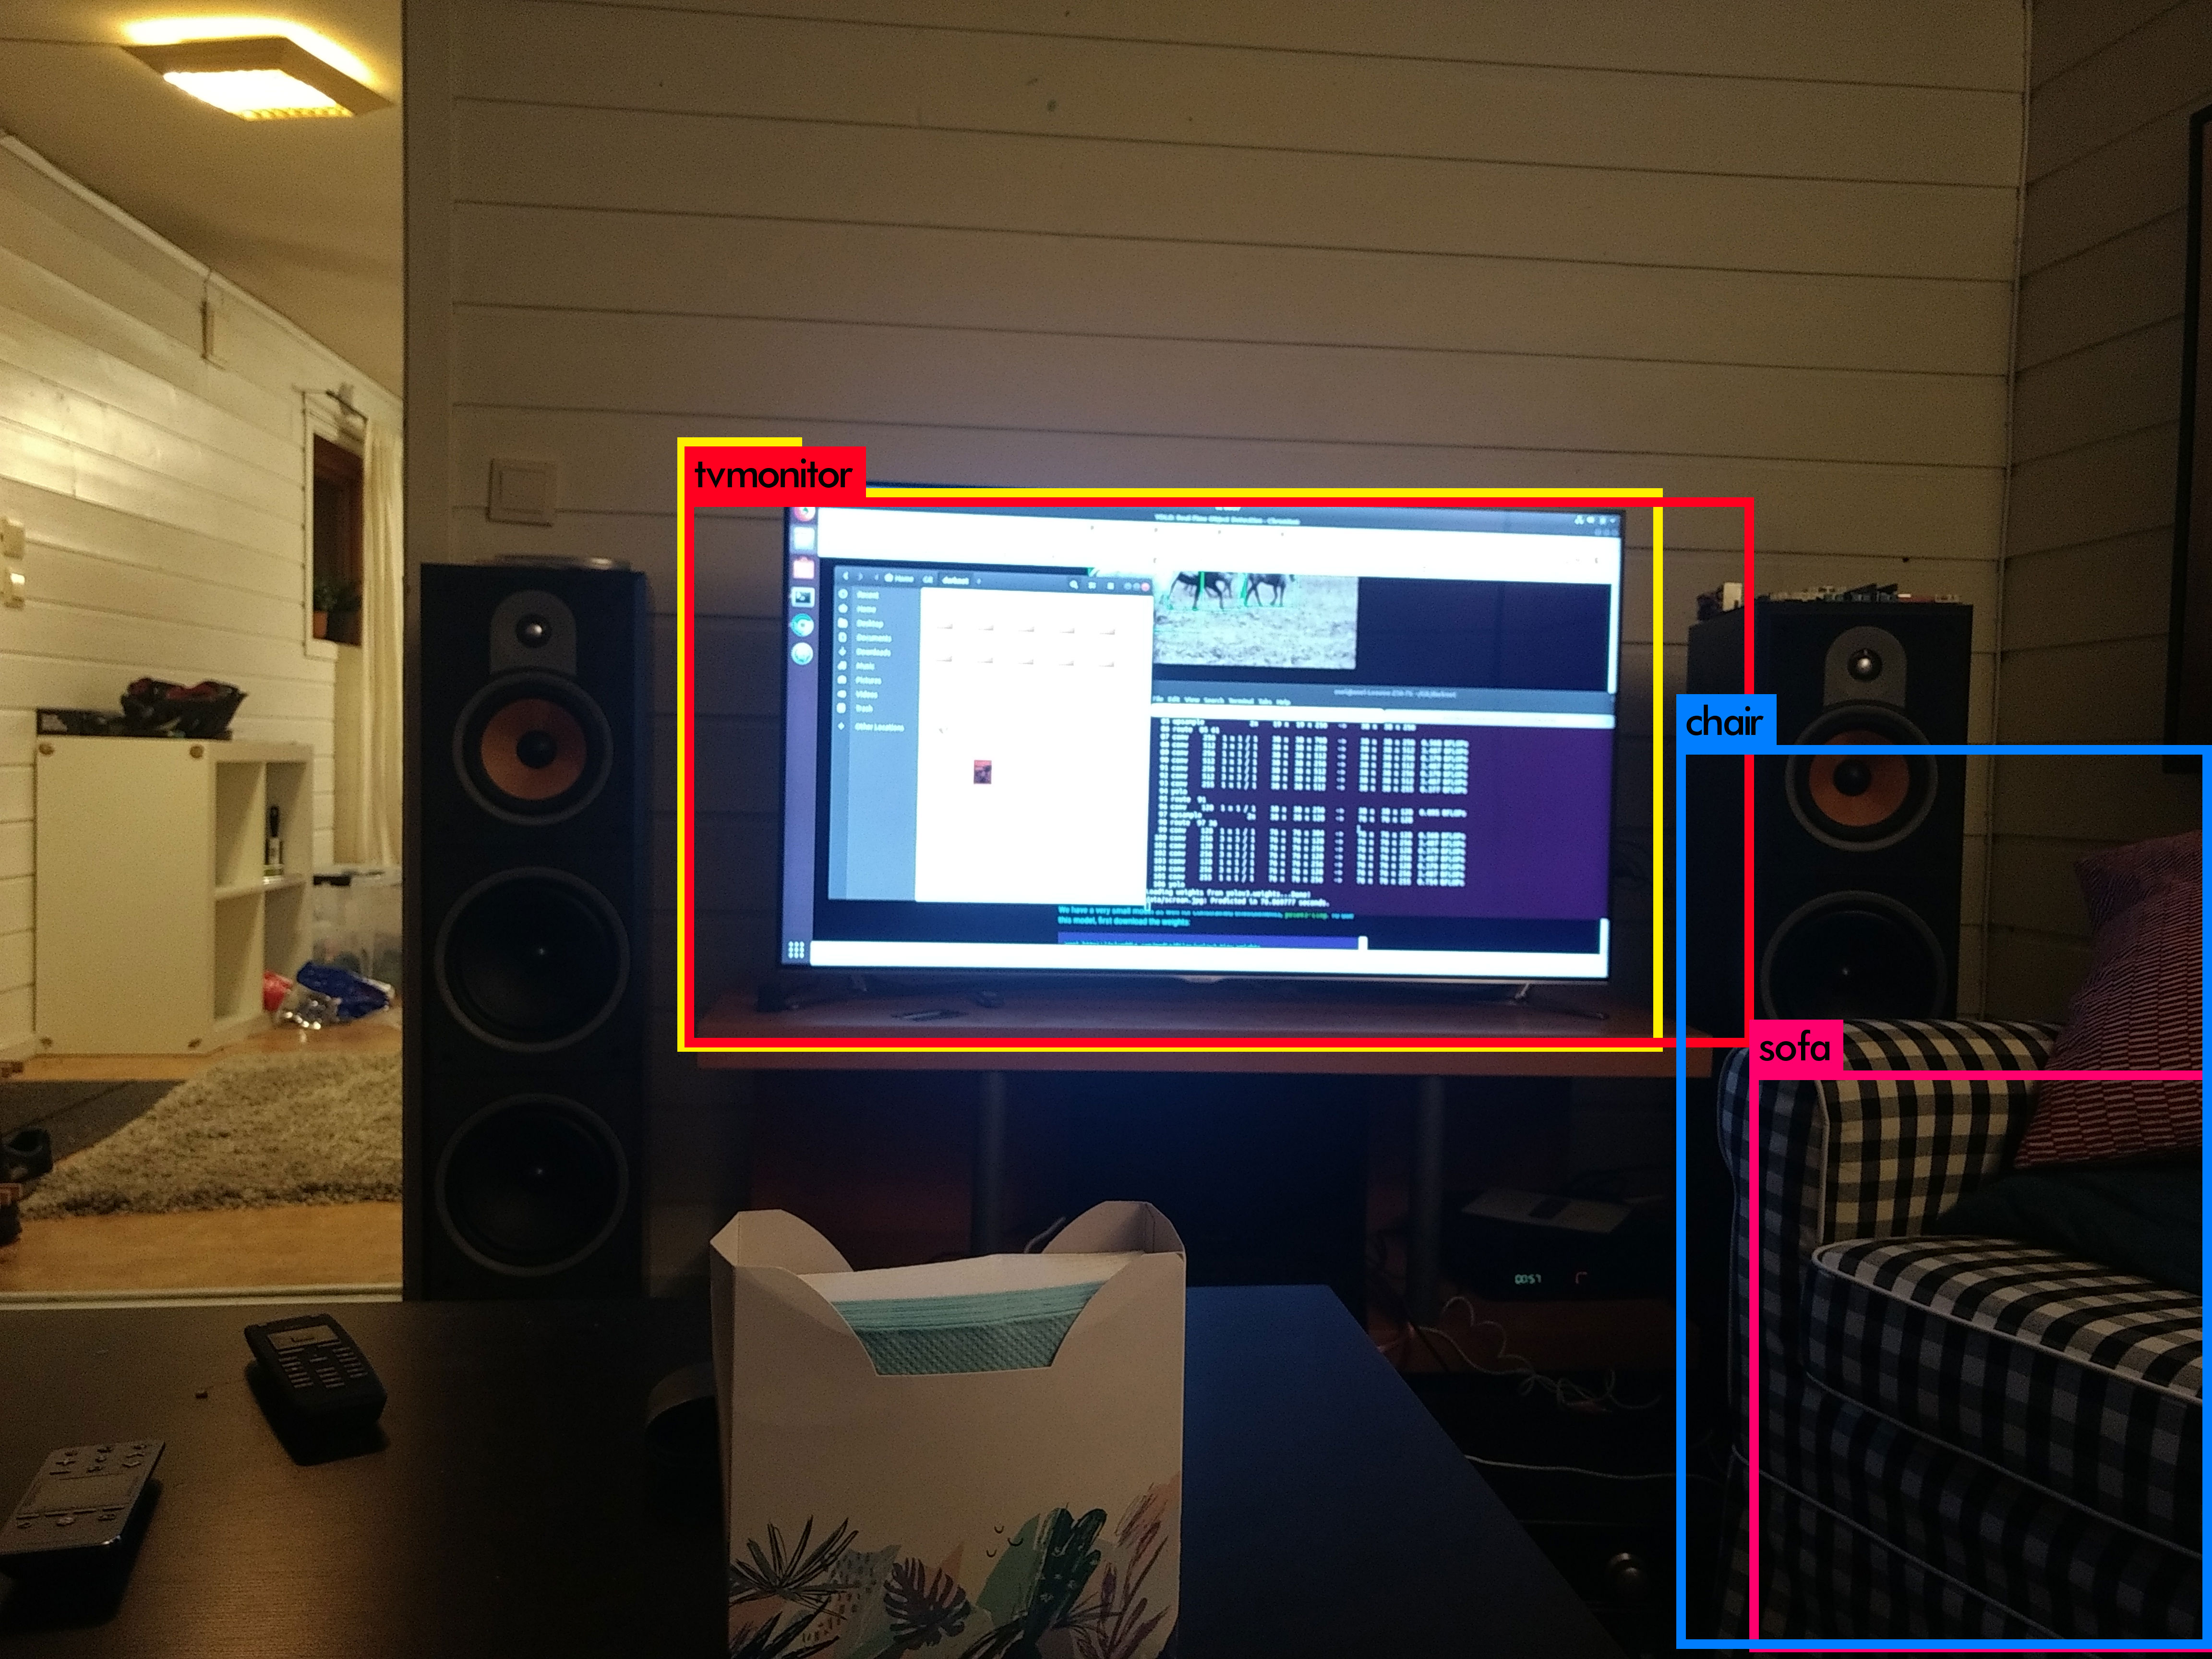
\includegraphics[width=10cm]{experiment_files/YOLOv3_tiny.jpg}
    \caption{Test result form YOLOv3-tiny }
    \label{fig:YOLOv3_tiny}
\end{figure}

\subsection*{YOLOv3-416}
One of the normal versions with a mid range resolution of 416x416.

Frame rate on fast GPU: 35 FPS \cite{yolo_res}.
\begin{lstlisting}[frame=single]
# Running YOLOv3-416 with threshold value of 10\% 
# Input:
 ./darknet detect cfg/yolov3.cfg yolov3_416.weights data/stue.jpg -thresh 0.1
 
#Output
data/stue.jpg: Predicted in 80.764753 seconds.
book: 21%
remote: 31%
tvmonitor: 100%
sofa: 93%
chair: 14%
\end{lstlisting}

\begin{figure}[hb]
    \centering
        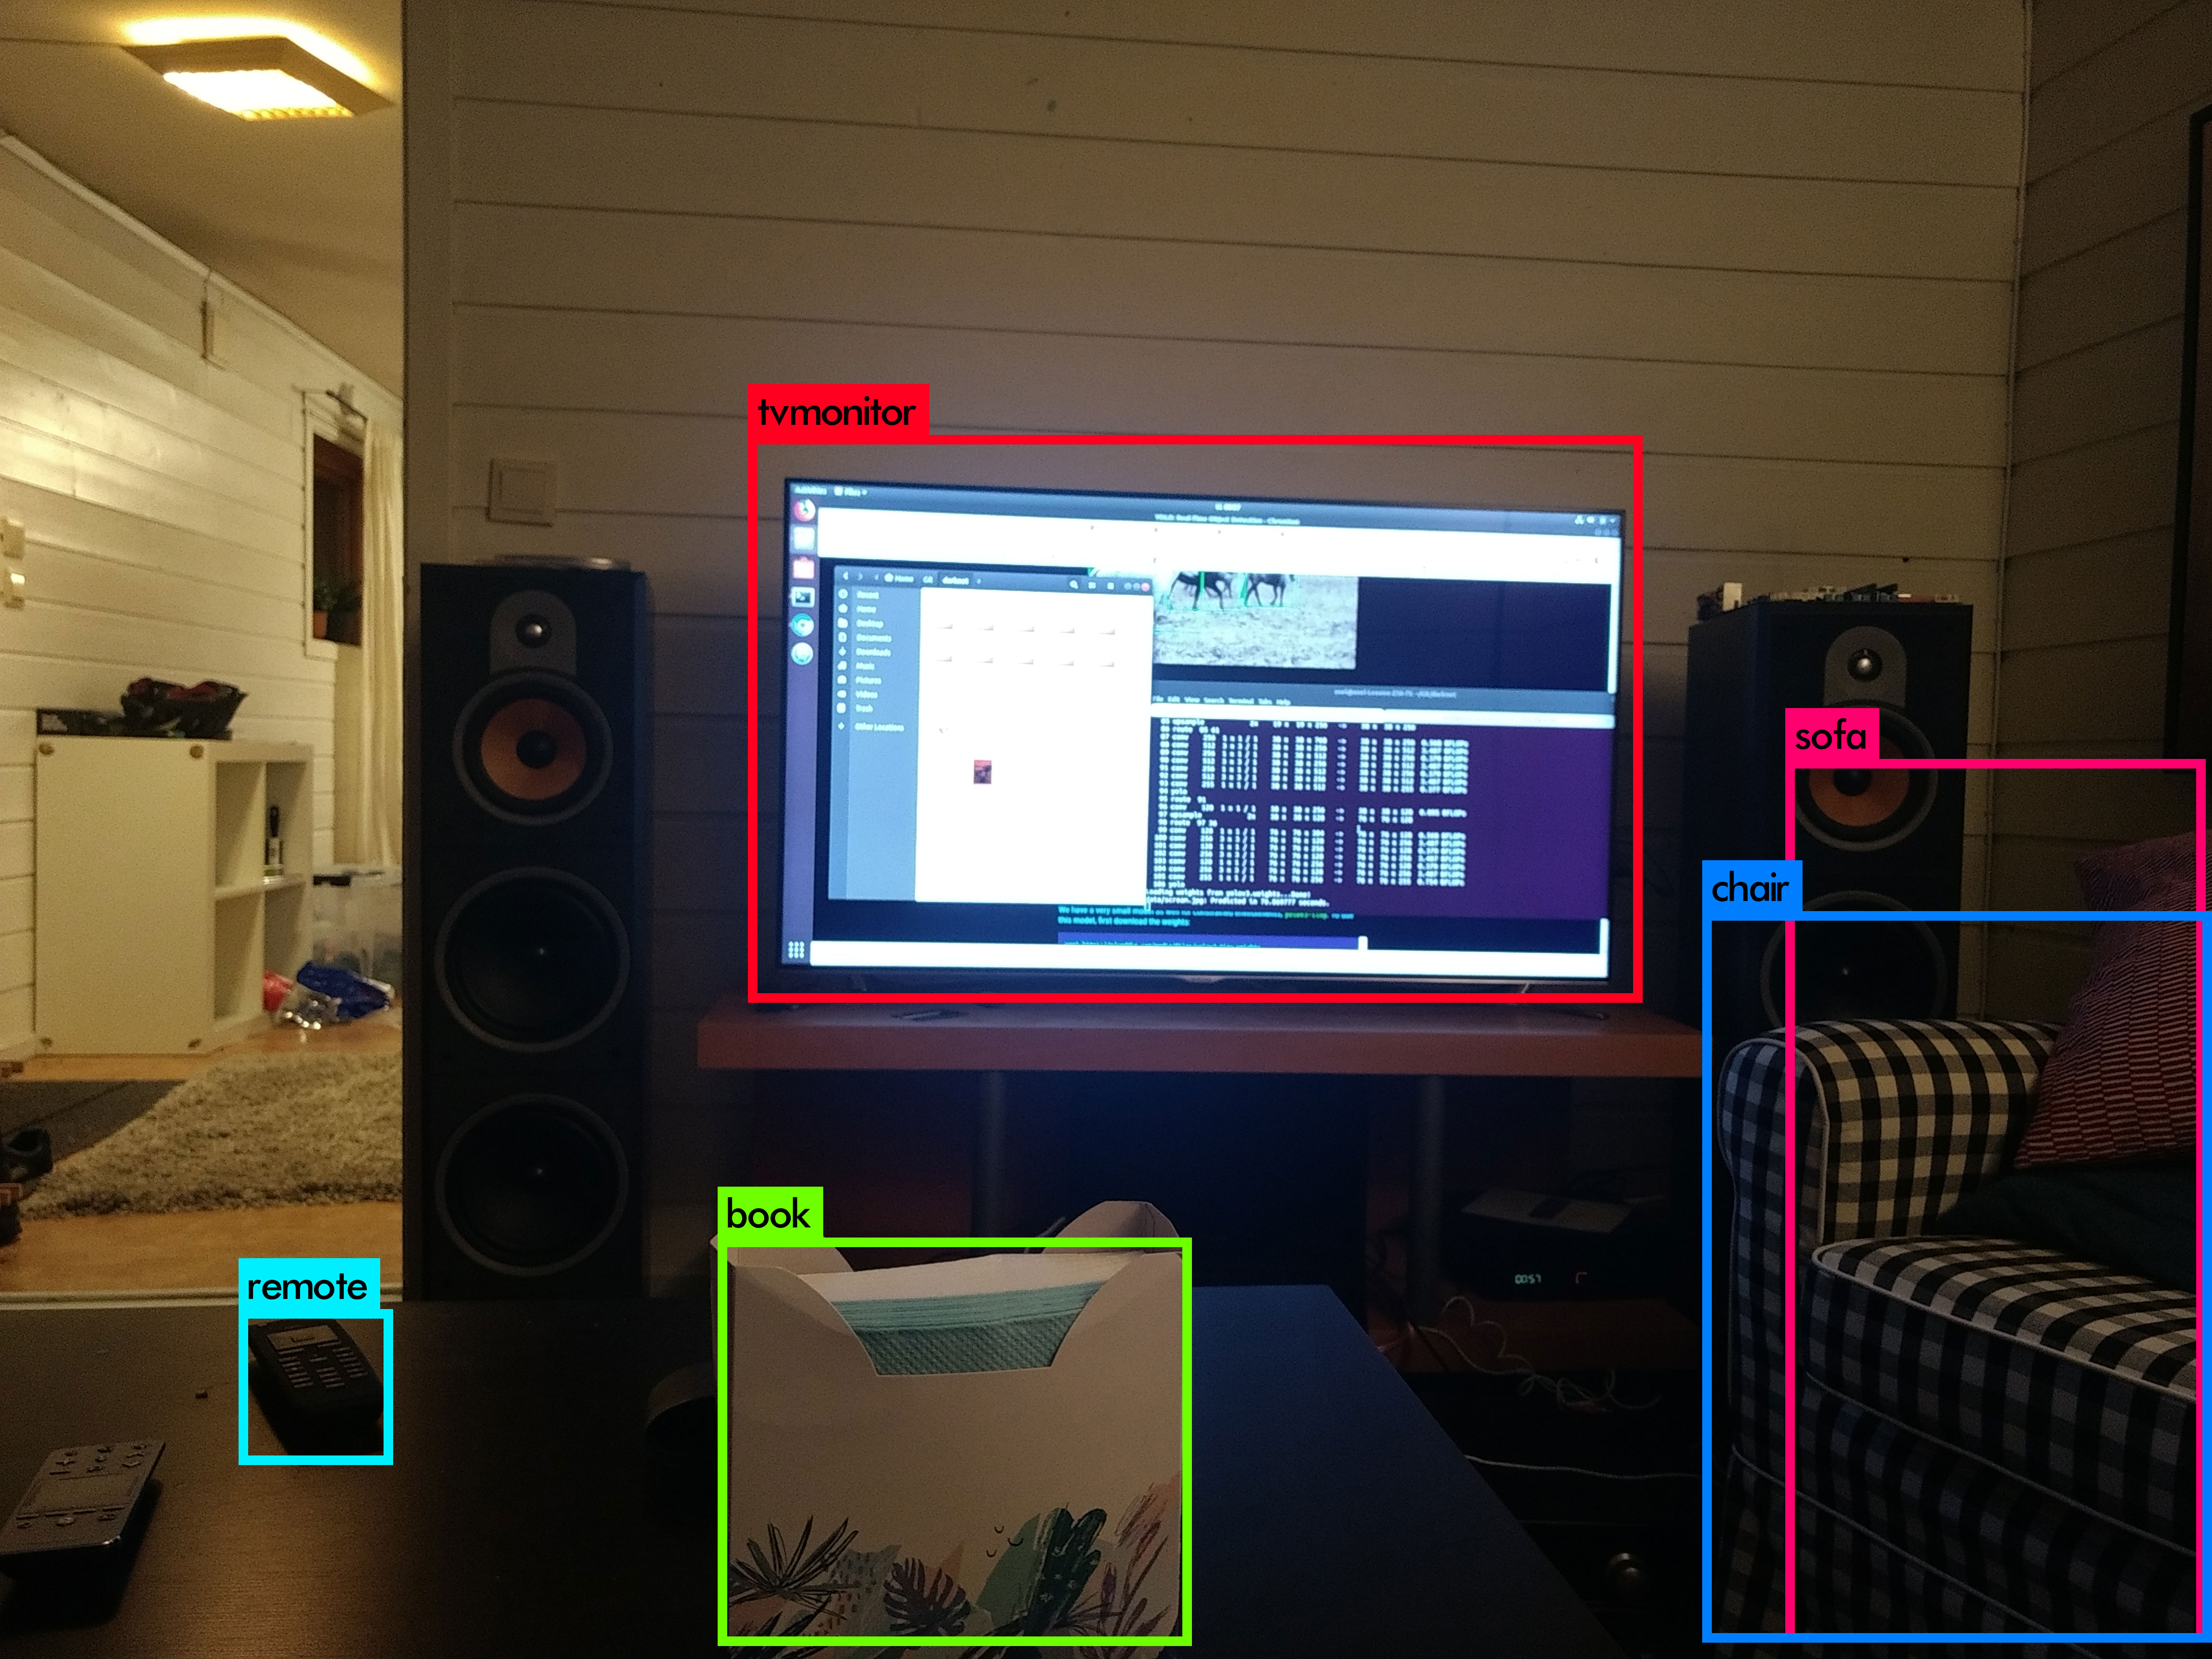
\includegraphics[width=10cm]{experiment_files/YOLOv3_416.jpg}
    \caption{Test result form YOLOv3-416}
    \label{fig:YOLOv3_416}
\end{figure}
\newpage
\subsection*{YOLOv3-spp}
The heaviest version, the YOLOv3-spp

Frame rate on fast GPU: 20 FPS \cite{yolo_res}.
\begin{lstlisting}[frame=single]
# Running YOLOv3_spp with threshold value of 10\% 
# Input:
./darknet detect cfg/yolov3-spp.cfg yolov3-spp.weights data/stue.jpg -thresh 0.1

#Output
data/stue.jpg: Predicted in 78.793520 seconds.
remote: 53%
remote: 43%
tvmonitor: 87%
laptop: 36%
sofa: 93%
\end{lstlisting}

\begin{figure}
    \centering
        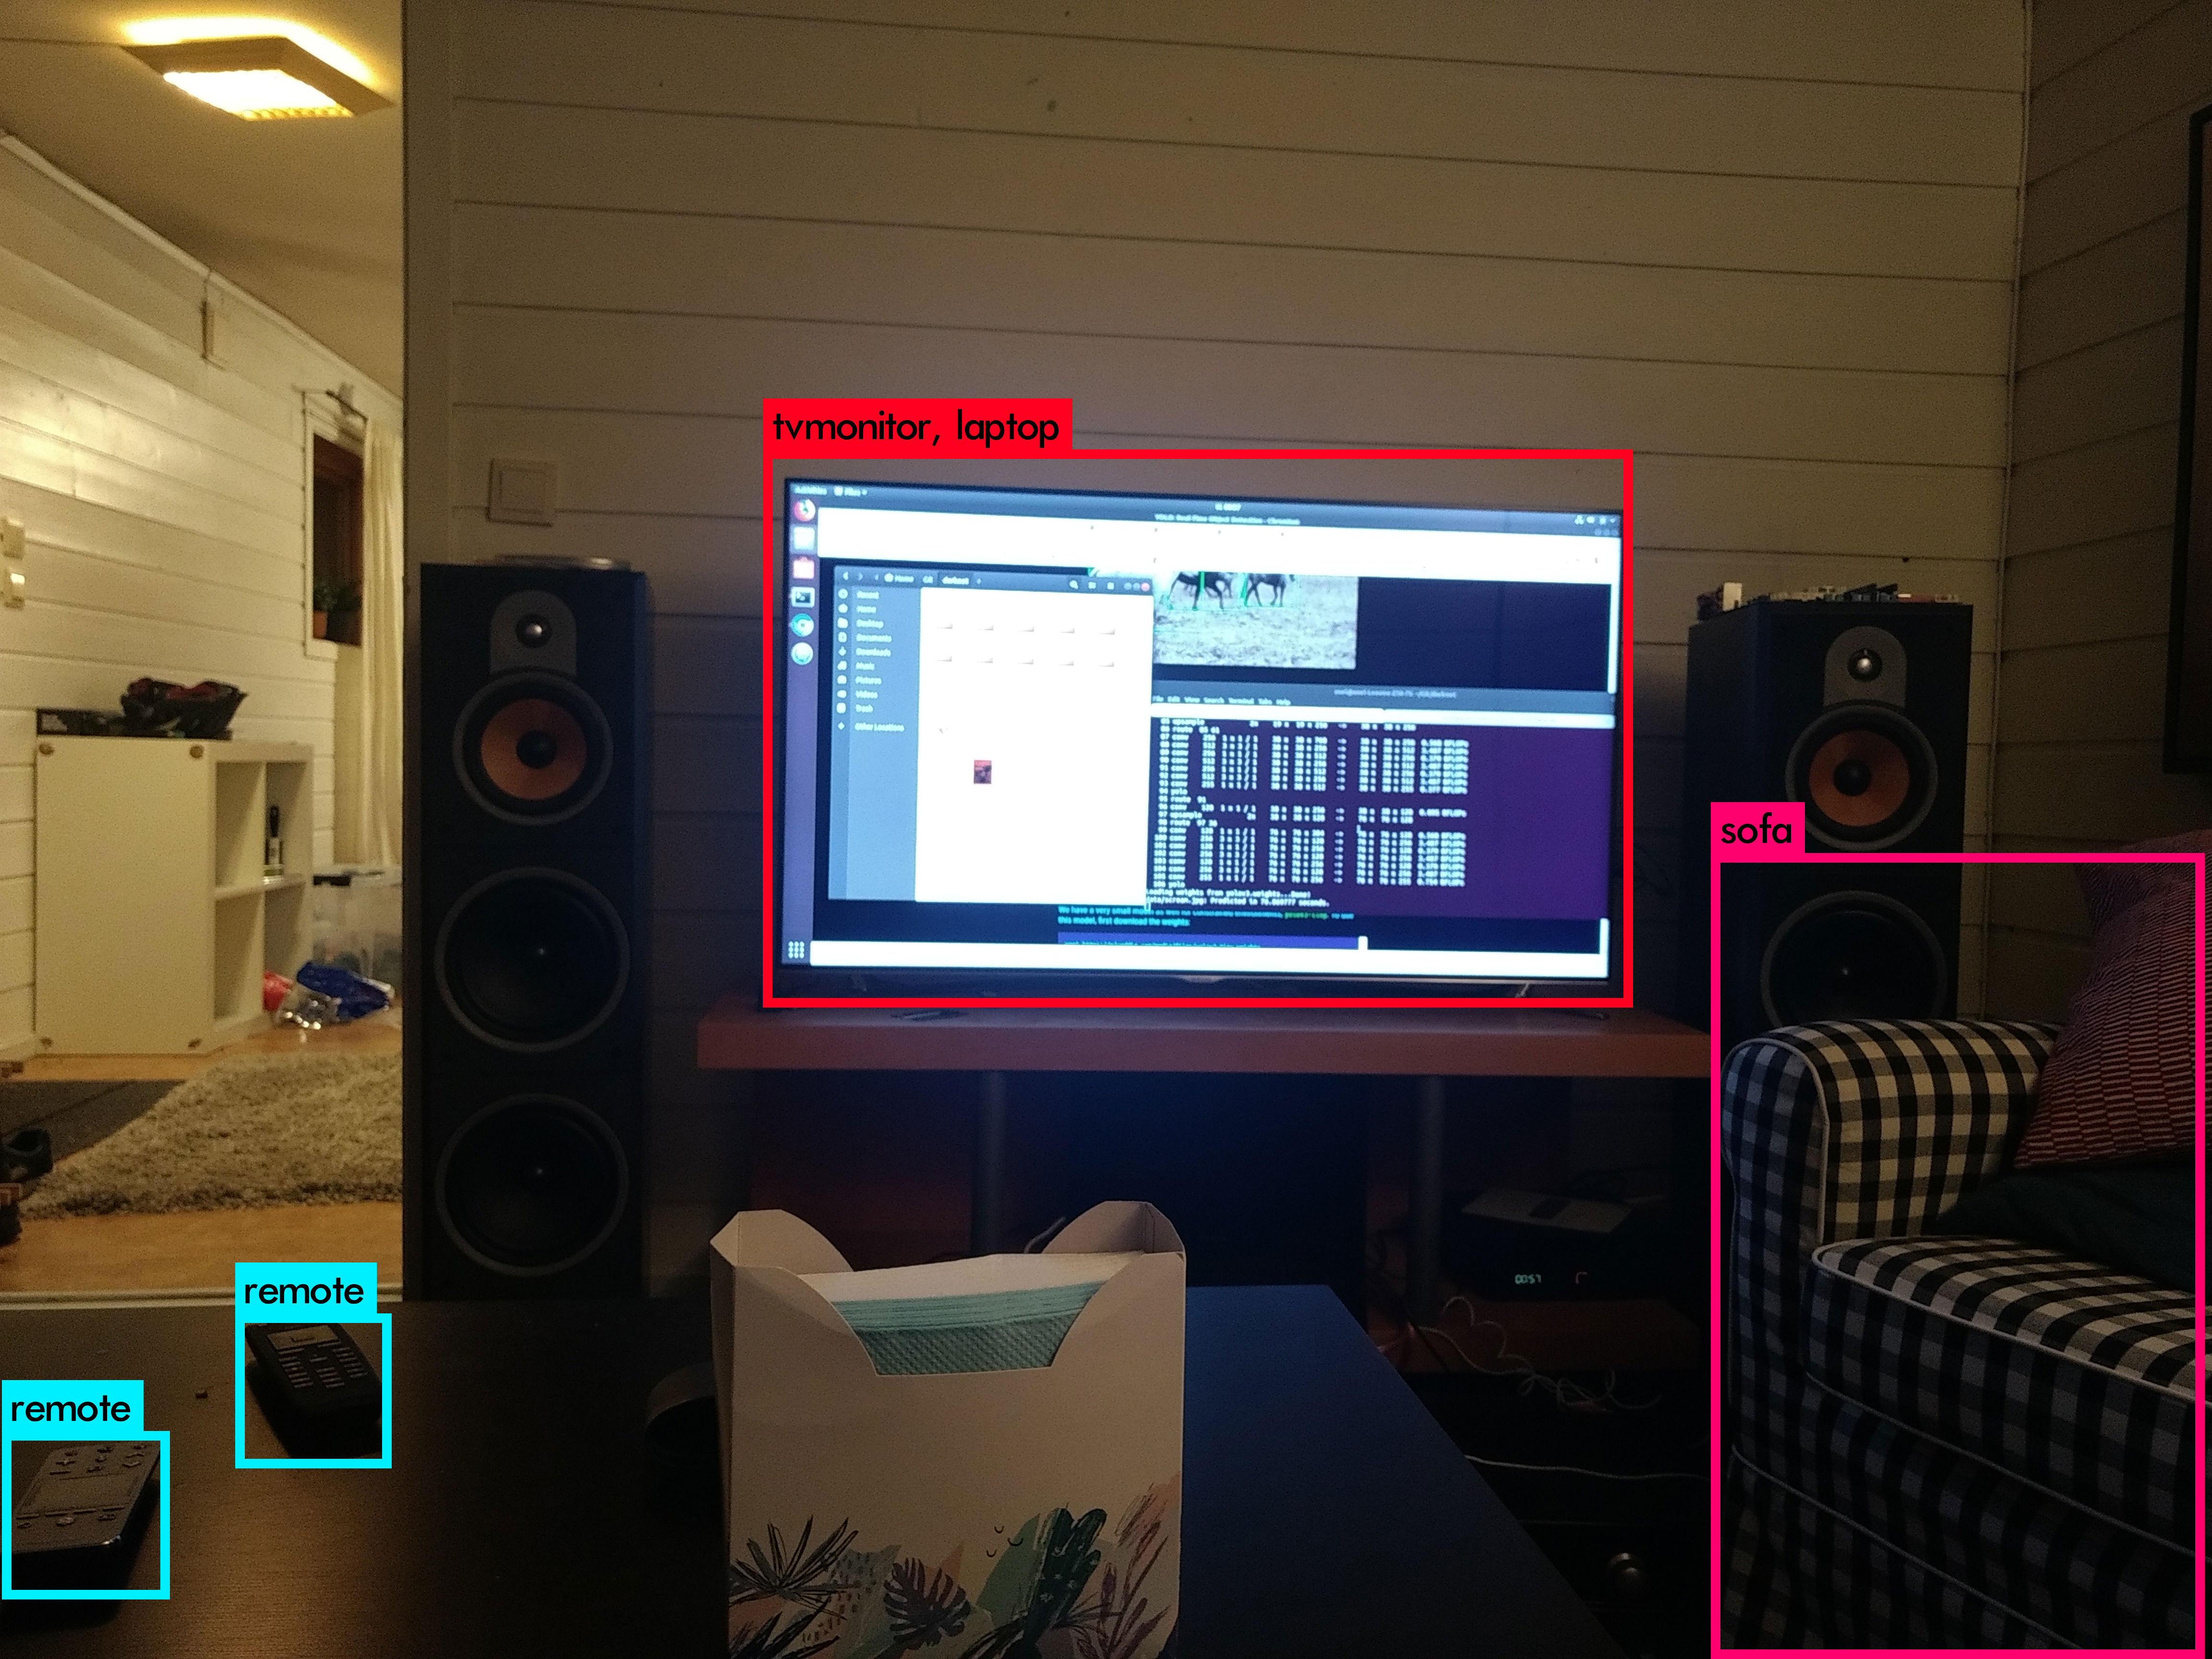
\includegraphics[width=10cm]{experiment_files/yolov3-spp.jpg}
    \caption{Test result form YOLOv3-spp}
    \label{fig:YOLOv3_spp}
\end{figure}

\subsection{Test Results}
After reviewing the test results, did all the different versions find some correct detections and some wrong detections.

\subsubsection*{Performance}
\begin{table}[]
\begin{tabular}{l|lll}
Model       & Test CPU time {[}s{]} & Cited time from GPU {[}FPS{]} & Cited mAP-50 score \cite{yolo_res} \\ \hline
YOLOv3-tiny & 3,29                  & 220                           & 33,1               \\
YOLOv3-416  & 80,76                 & 35                            & 55,3               \\
YOLOv3-spp  & 78,79                 & 20                            & 60,3              
\end{tabular}
\caption{My own test result compared to cited performance.}
\end{table}

The test results from the test, shown in table 1 differ performance wise, when comparing the cited GPU time from the tested CPU time for the picture to render. Most remarkable is the speed difference between the normal and the tiny CNN architecture. 3 against 80 second to render an image is quite the big difference. Also the YOLOv3-416 and the YOLOv3-spp had almost the same run time on CPU and on GPU the spp version is roughly 75\% slower then the 416 version. The difference of 2 secunds on the CPU runtime is negotiable, since there is other programs on the computer also using the CPU. The runtime differed between 70-80, when multiple test where run.

However this algorithm is designed as a real time detection algorithm, and test result prove that it is not possible to do real time usage of this algorithm if the test PC does not have a GPU with CUDA cores. But it works fine to do image detection, since run time is not that important.

\subsubsection*{Accuracy}
\begin{table}[]
\begin{tabular}{l|lllllll}
Model \textbackslash Detections {[}\%{]} & TV-monitor & Sofa & Remote 1 & Remote 2 & Book {[}fp{]} & Laptop {[}fp{]} & Chair {[}fp{]} \\ \hline
YOLOv3-tiny                              & 73         & 16   & N/A      & N/A      & N/A                       & 49                          & 18                         \\
YOLOv3-416                               & 100        & 93   & 31       & N/A      & 21                        & N/A                         & 14                         \\
YOLOv3-spp                               & 87         & 93   & 53       & 43       & N/A                       & 36                          & N/A                       
\end{tabular}
\caption{Test results in detecting different objects, including fp (false positives)}
\end{table}
Looking at table 2.
As expected, the tiny version did not perform that well in case of detection accuracy, but it did manage to find the two correct objects, though the confidence score of only 16\% prove it was not certain at all. With a higher threshold, tiny would not detect it at all. 
The YOLOv3-416 and spp, did archived an higher accuracy, but non of them had a 100\% detection rate. The 416 was the only to detect the TV as only a TV, but on all other objects, the spp were quite successfully. 